\documentclass[12pt]{article}

%packages
\usepackage{fancyhdr}
\usepackage[margin=1in]{geometry}
\usepackage[utf8]{inputenc}
\usepackage{listings}
\usepackage{booktabs}
\usepackage{enumitem}
\usepackage{pdfpages}
\usepackage{graphicx}
\usepackage{listings}
\usepackage{xcolor}
\usepackage{subcaption}
\usepackage{float}
\usepackage{amsmath}

%fancyheadr fix
\setlength{\headheight}{15pt}

%commands to lslistings
\lstset{
    basicstyle=\ttfamily\small,
    breaklines=true,     
    breakatwhitespace=true,
    frame=single,
    numbers=left,
    numberstyle=\tiny,
    columns=fullflexible,
    keepspaces=true
}


%title info
\newcommand{\doctitle}{STA 5635 HW 7}
\newcommand{\name}{Palmer Swanson}
\newcommand{\docdate}{\today}

%document
\begin{document}

\begin{center}
    {\Large \doctitle}\\[6pt]
    {\name}\\[3pt]
    {\docdate}
\end{center}
\vspace{12pt}

\section*{Problem 1}

\begin{enumerate}[label=(1\alph*), ref=1\alph*]
    \item NN w/ one hidden layer, 256 neurons, ReLU activation.
    \begin{figure}[htbp] 
        \centering 
        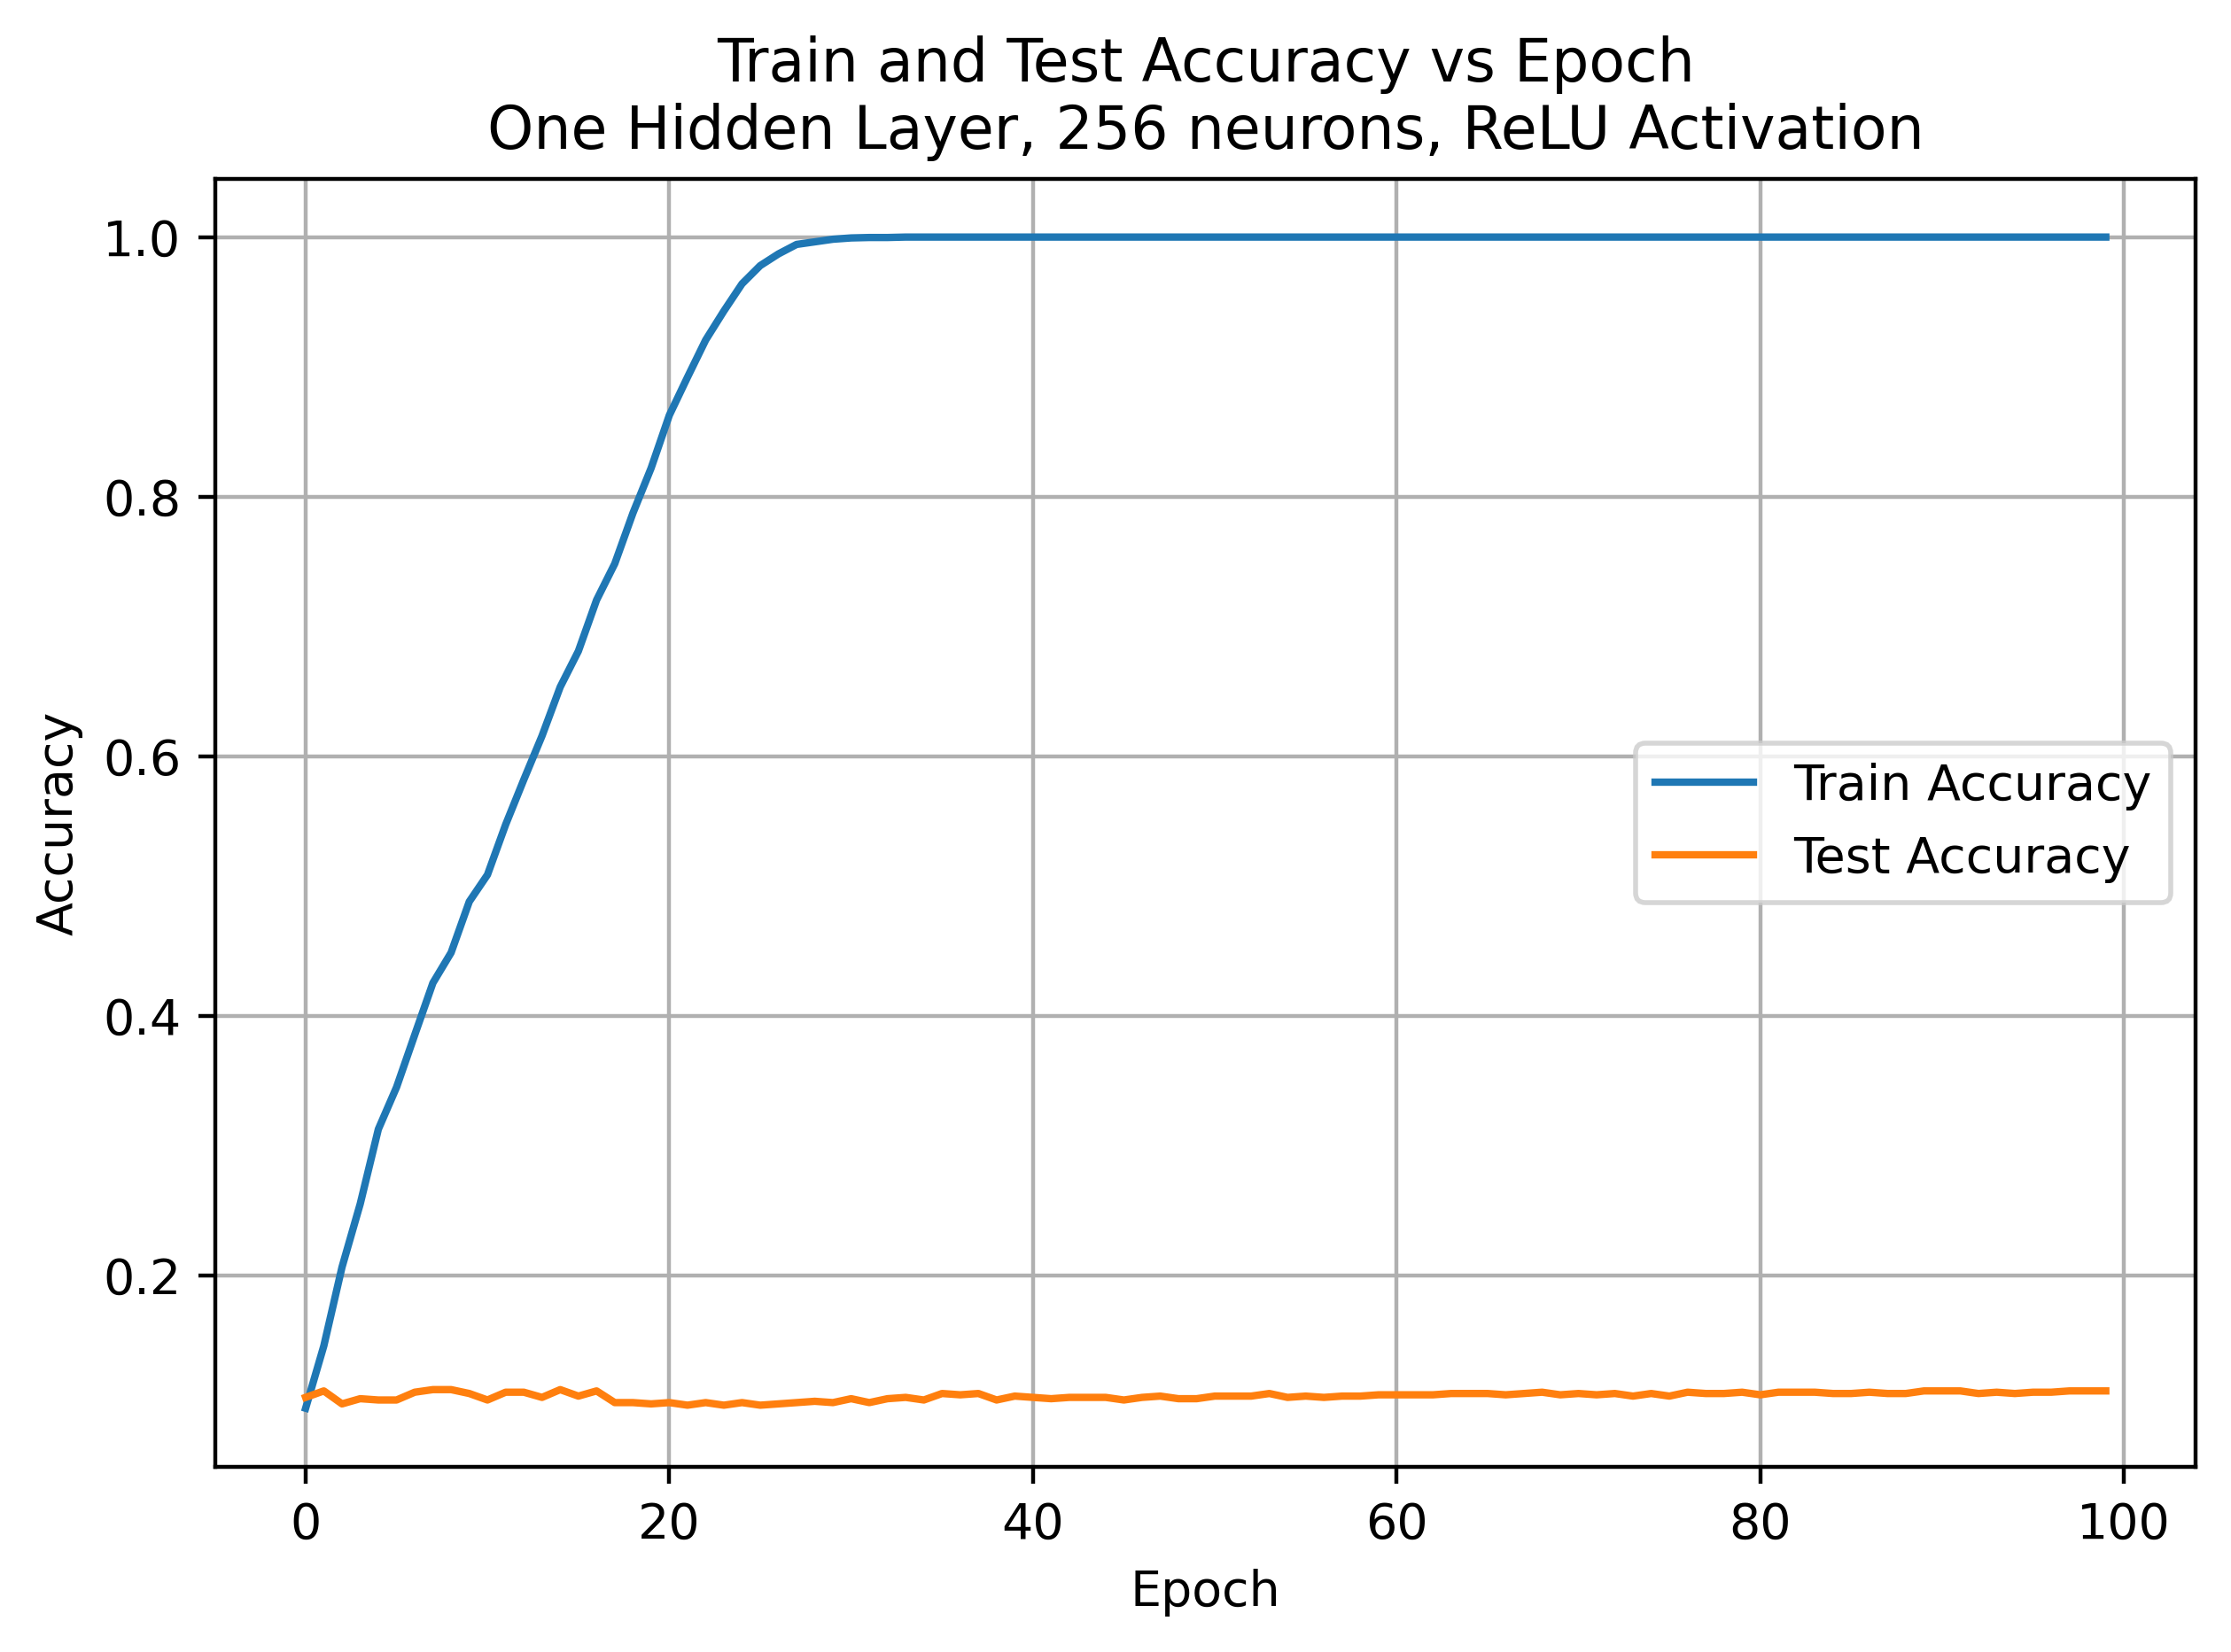
\includegraphics[width=0.5\linewidth]{../figures/part_a.png} 
        \caption{Train and Test accuracy vs. Epoch, part a.} 
    \label{fig:part a} 
    \end{figure}
    \item NN w/ two hidden laters, 64 neurons, ReLU activation
    \begin{figure}[htbp] 
        \centering 
        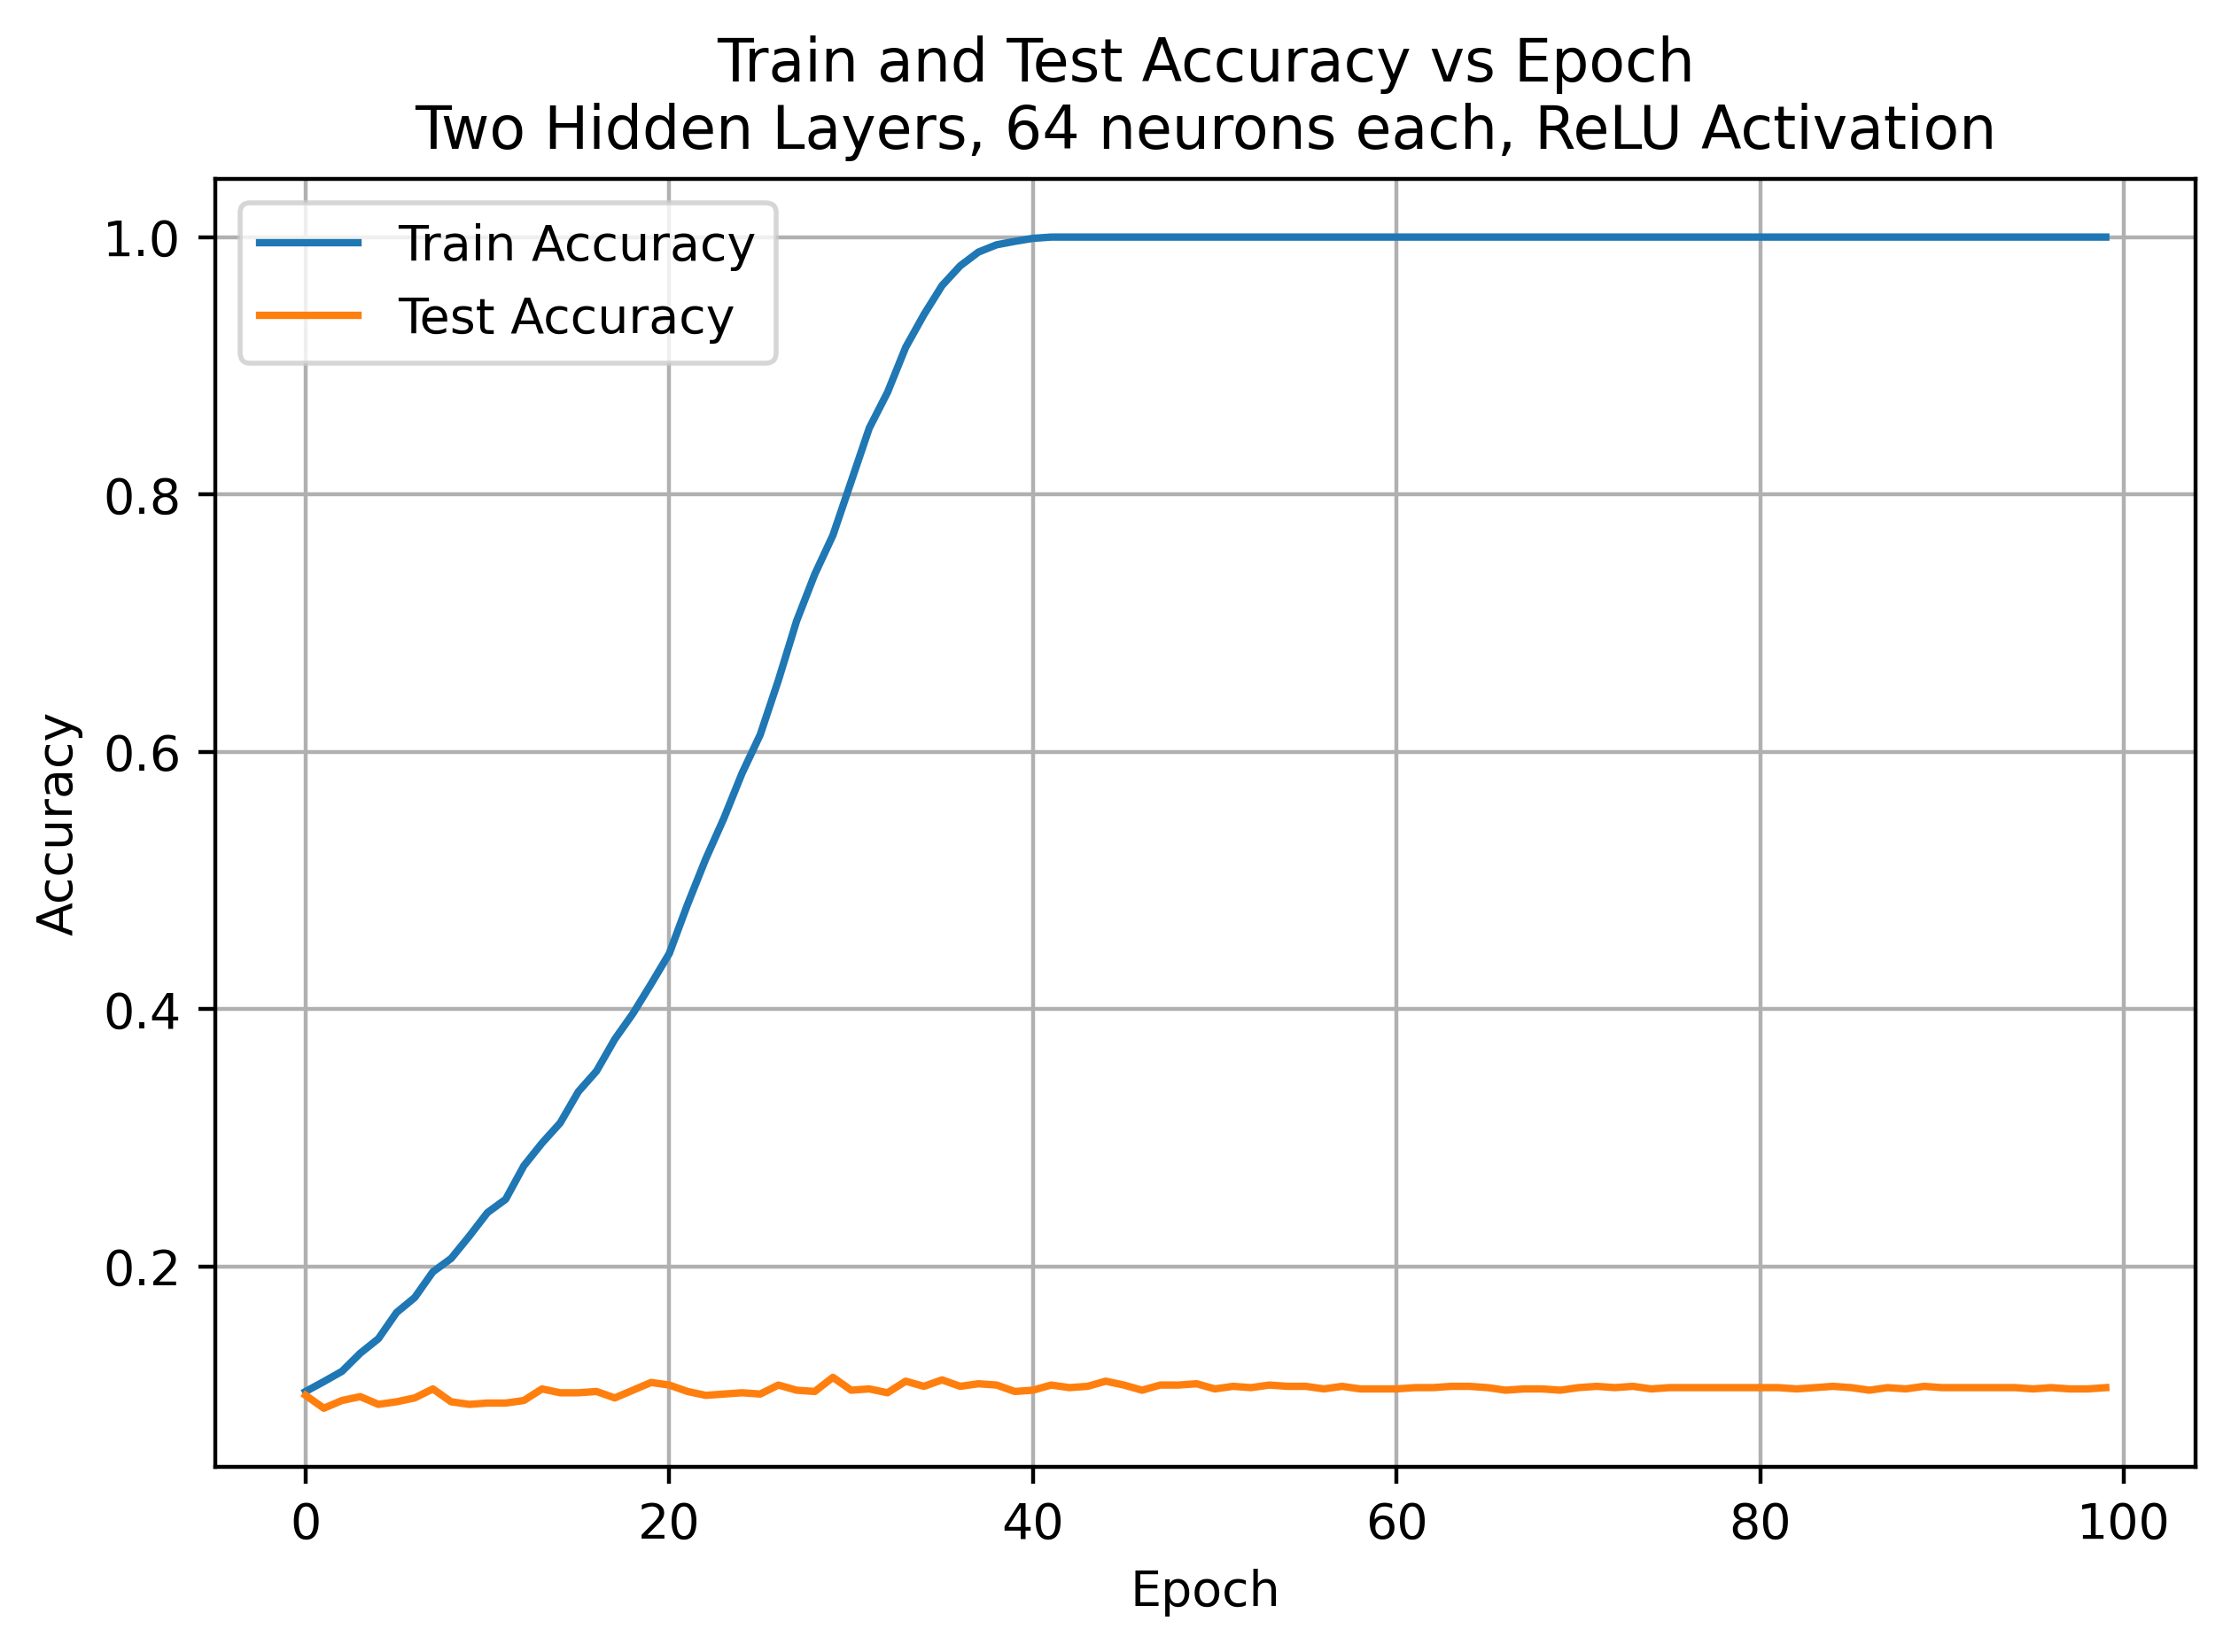
\includegraphics[width=0.5\linewidth]{../figures/part_b.png} 
        \caption{Train and Test accuracy vs. Epoch, part b.} 
    \label{fig:part b} 
    \end{figure}
    \item NN w/ one hidden layer, 256 neurons, ReLU activation.
    \begin{figure}[htbp] 
        \centering 
        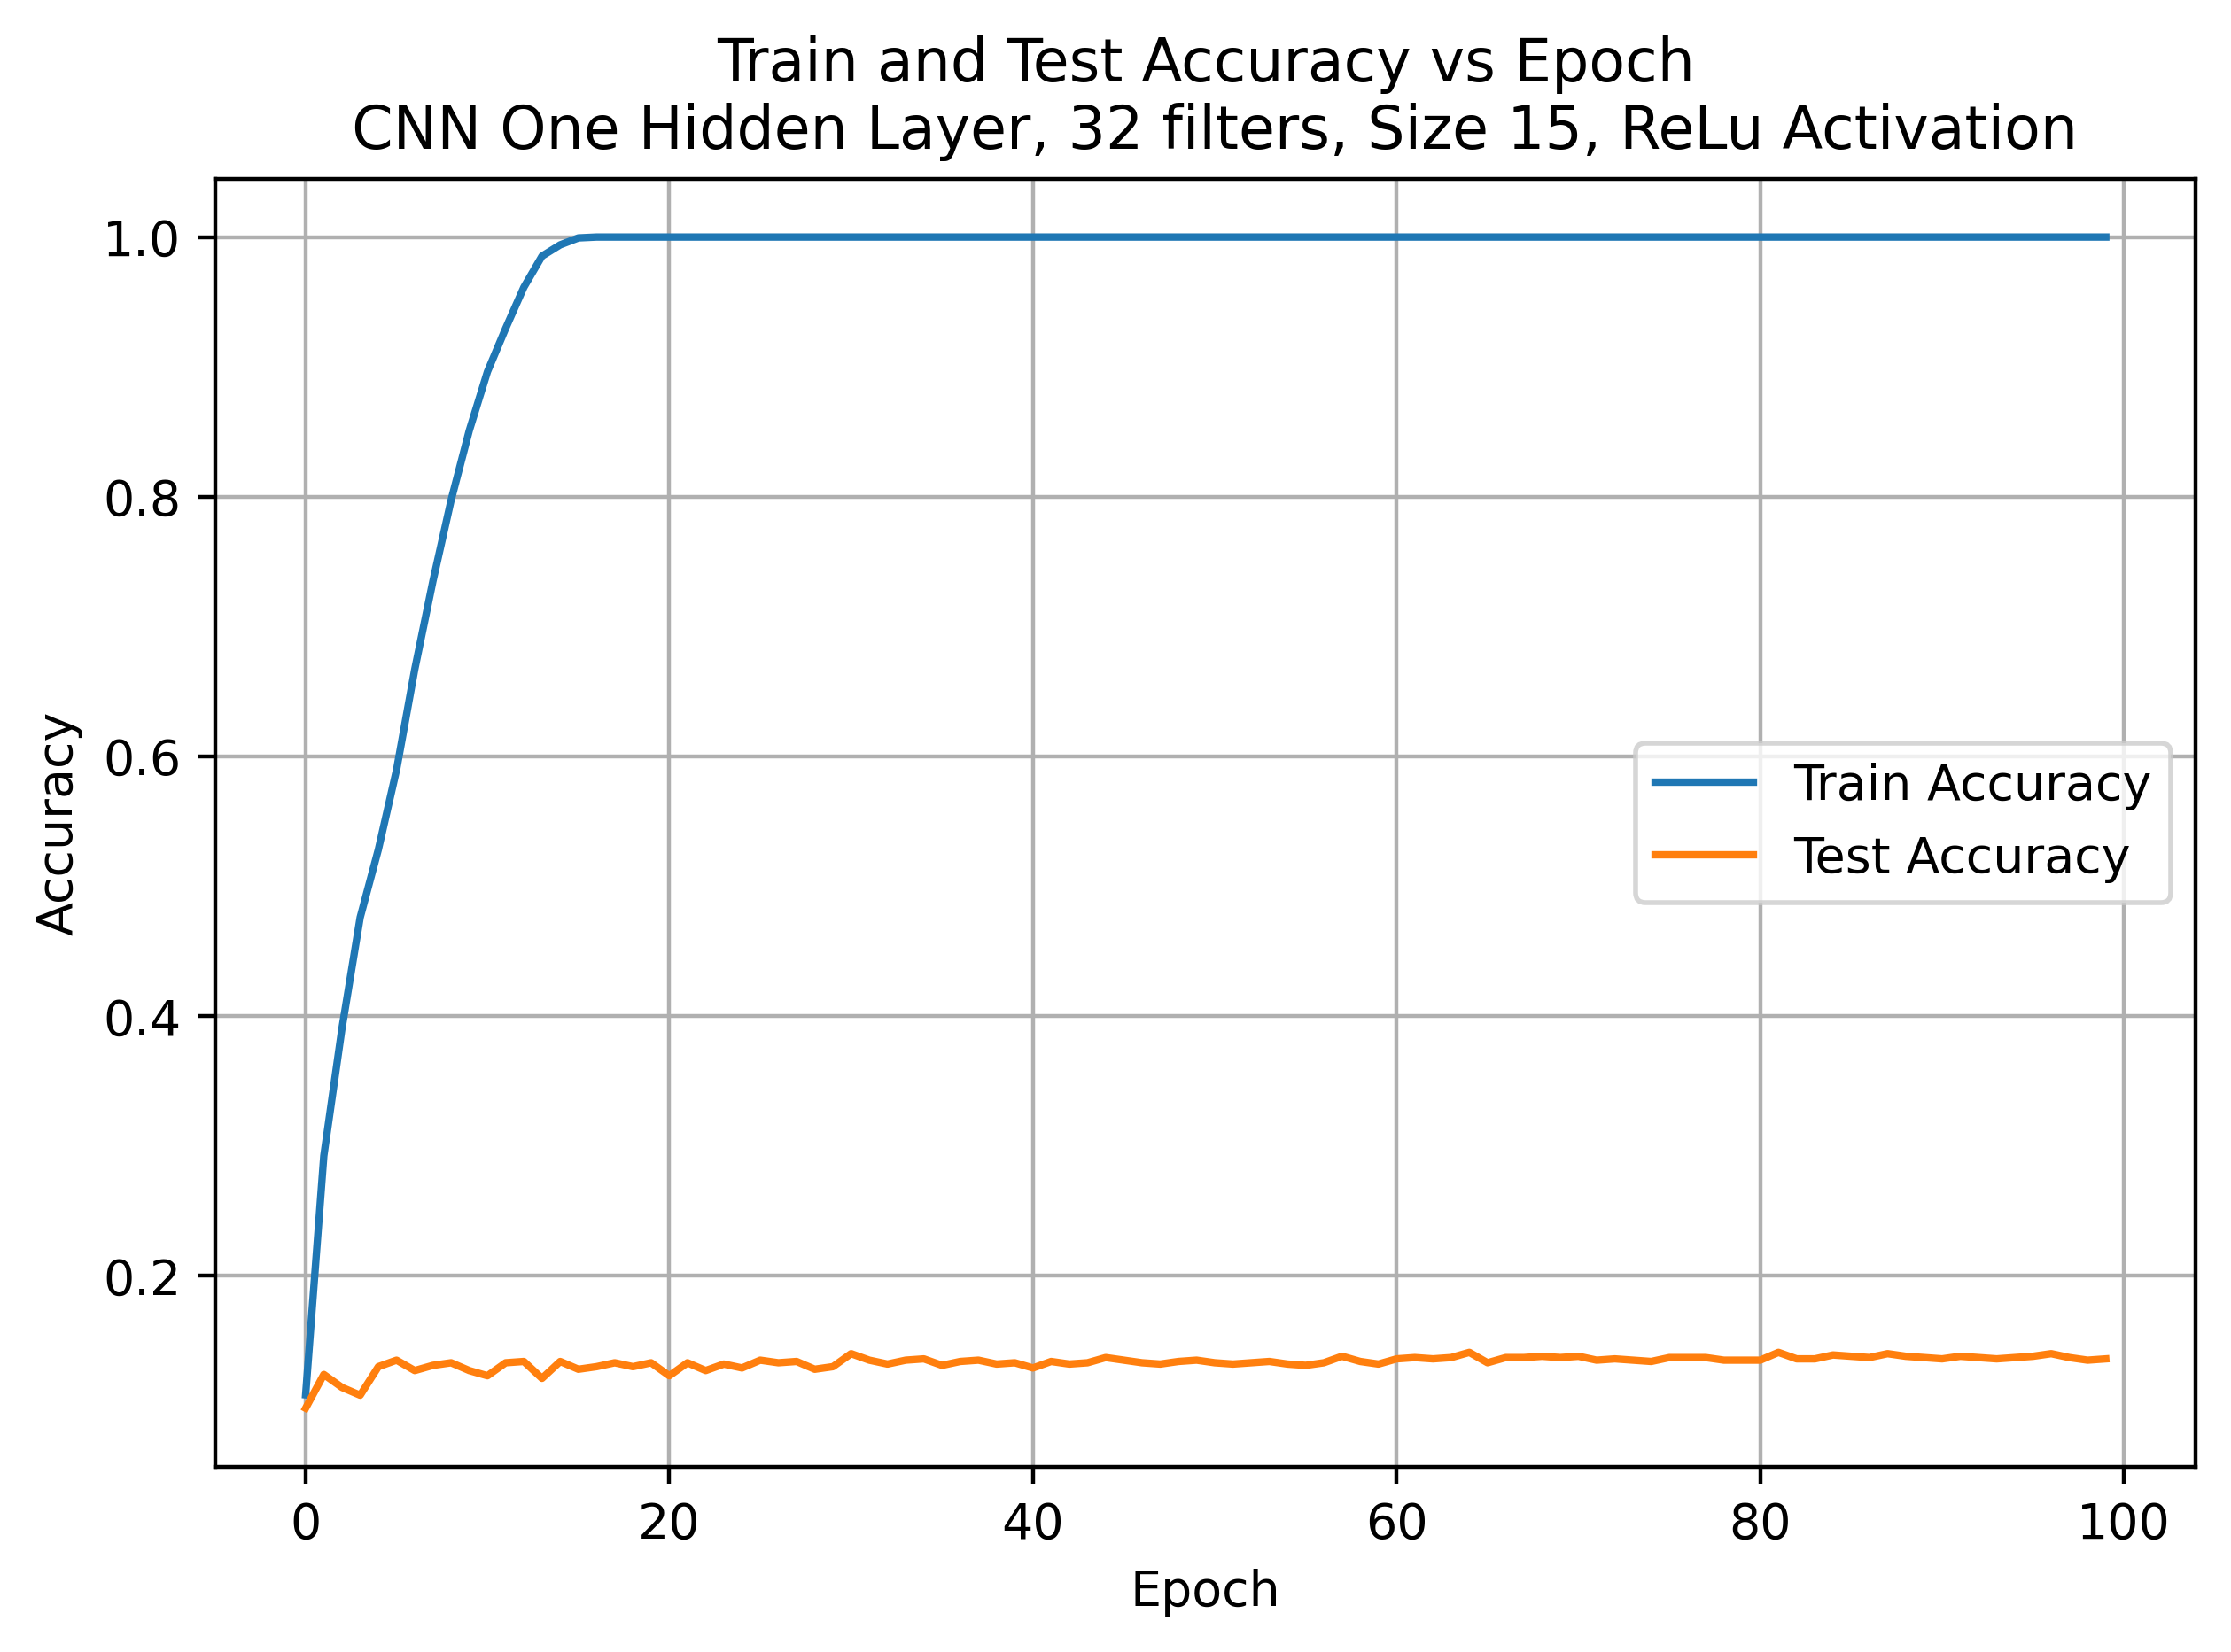
\includegraphics[width=0.5\linewidth]{../figures/part_c.png} 
        \caption{Train and Test accuracy vs. Epoch, part c.} 
    \label{fig:part c} 
    \end{figure}
    \item CNN w/ one hidden layer, 32 filters of size 15, ReLU activation
    \begin{figure}[htbp] 
        \centering 
        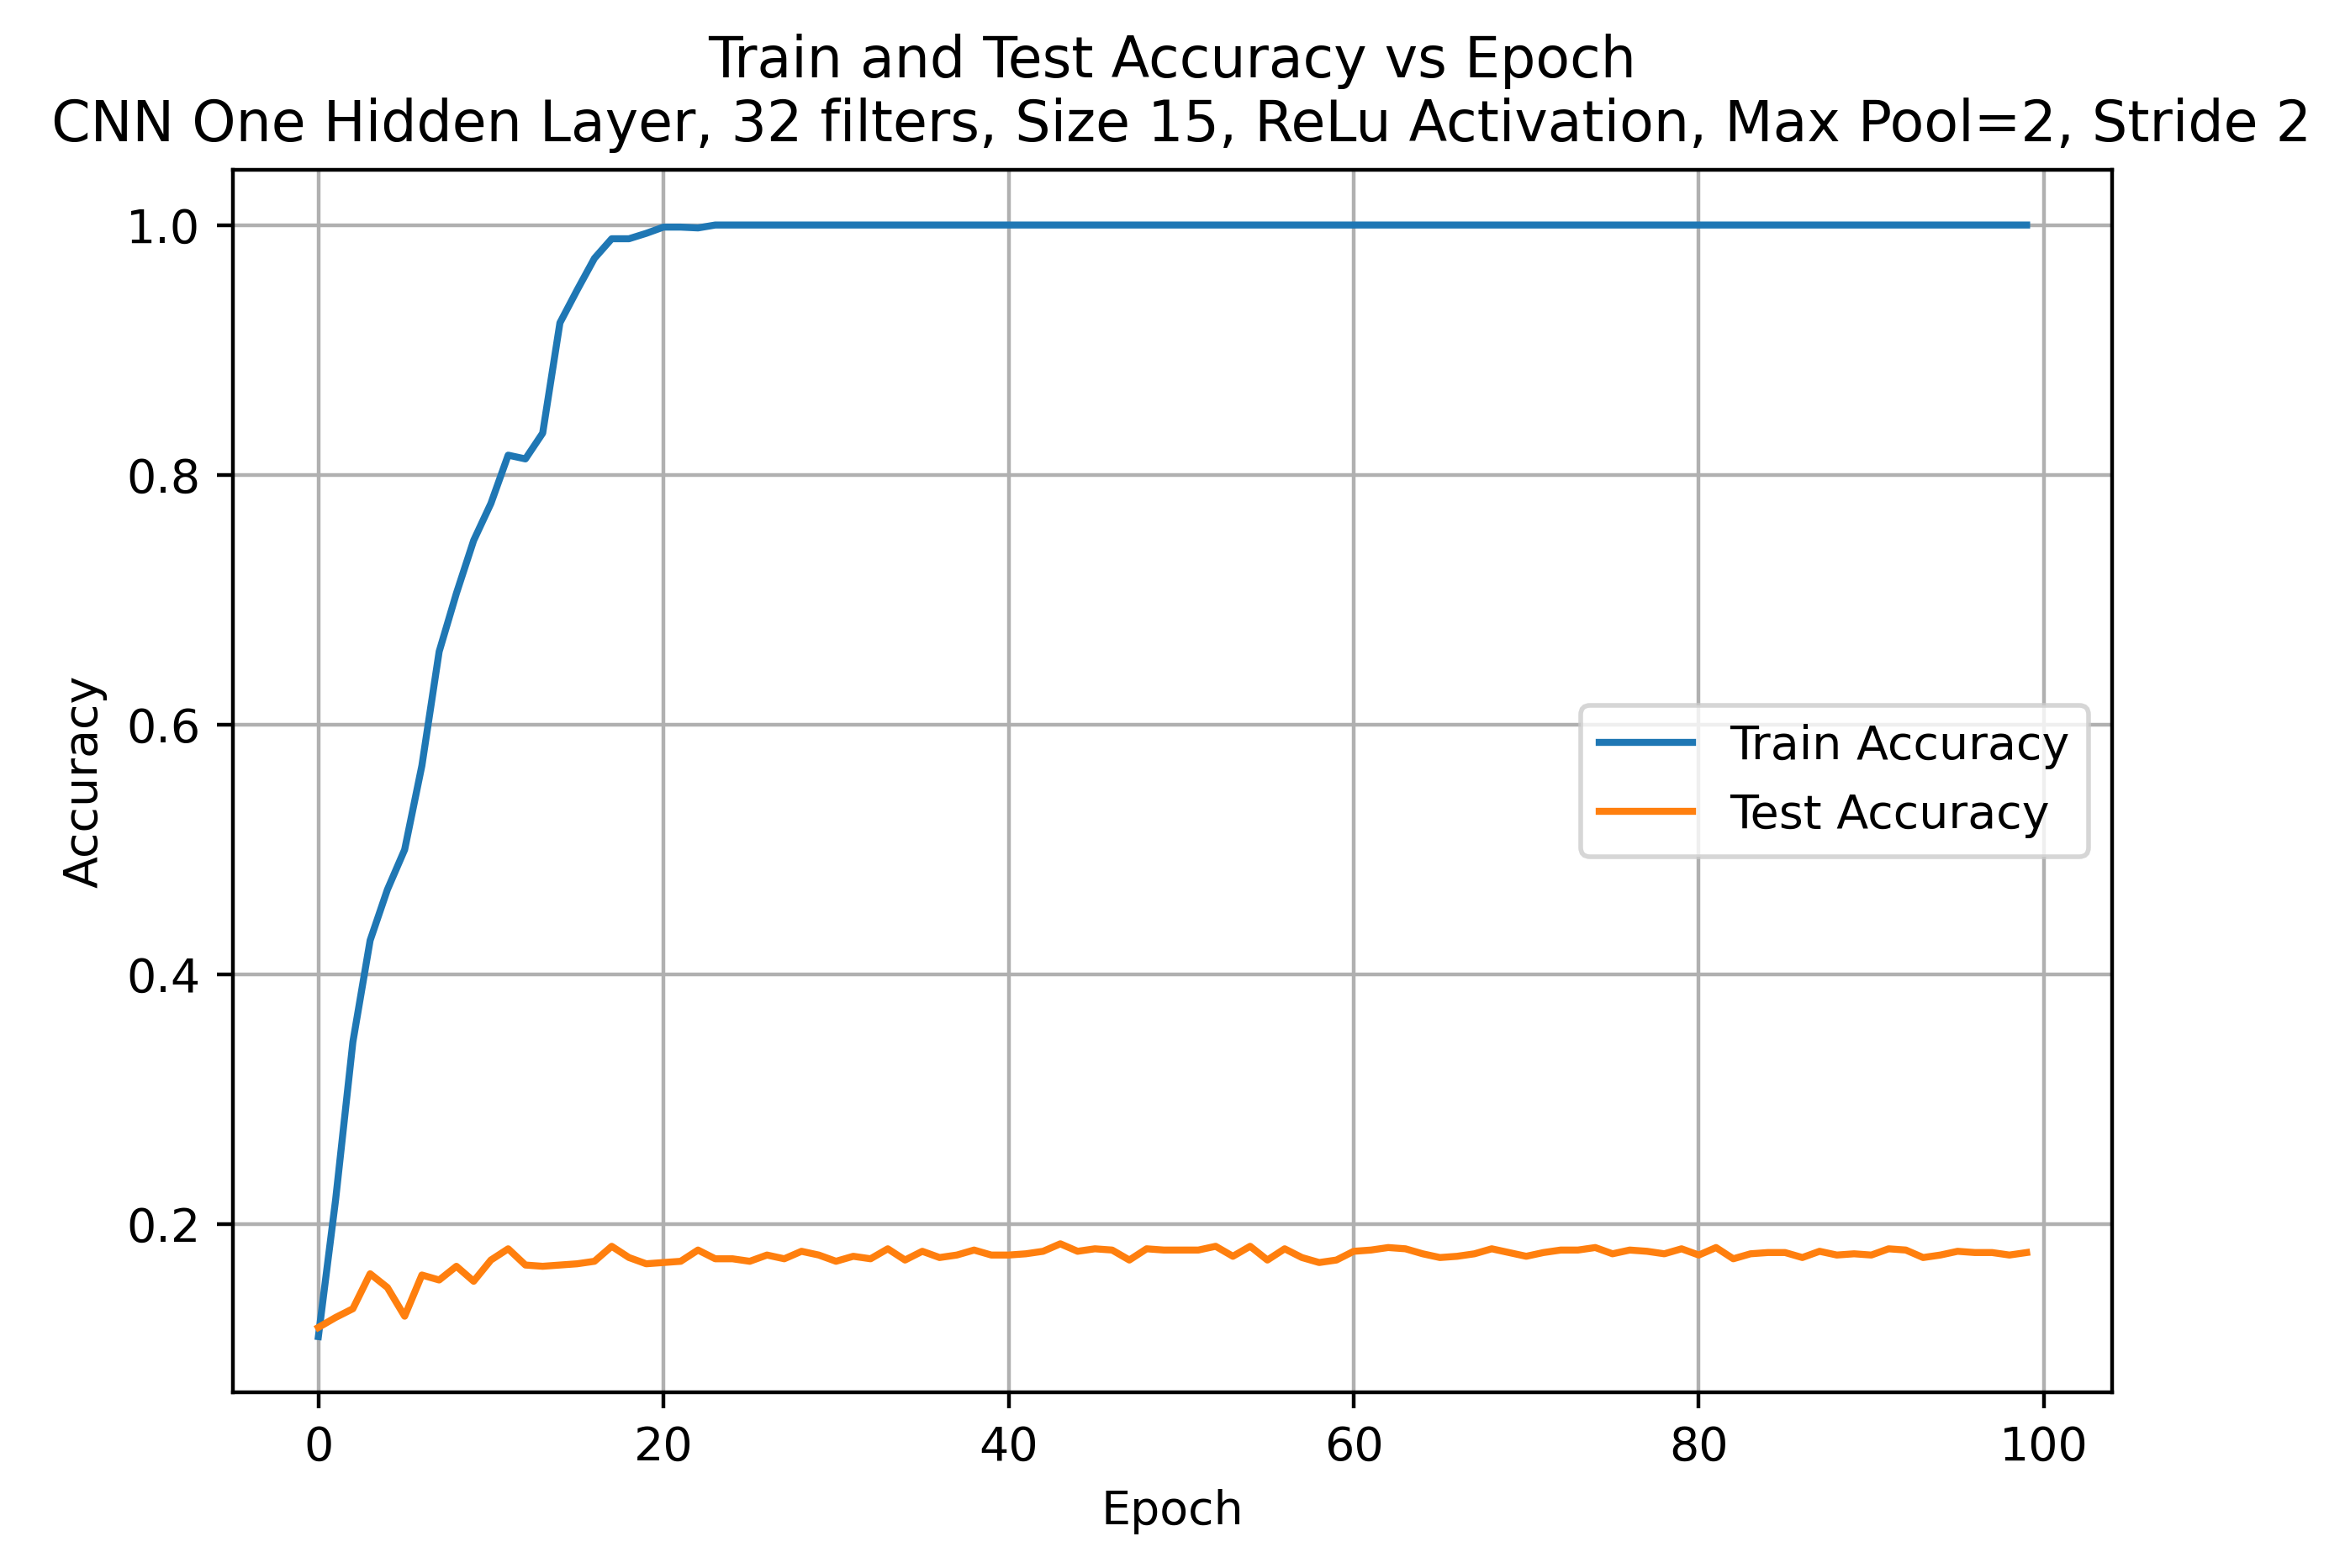
\includegraphics[width=0.5\linewidth]{../figures/part_d.png} 
        \caption{Train and Test accuracy vs. Epoch, part d.} 
    \label{fig:part d} 
    \end{figure}
    \item CNN w/ one hidden layer, 32 filters of size 15, ReLUE activation, max pooling size 2, stride 2.
    \begin{figure}[htbp] 
        \centering 
        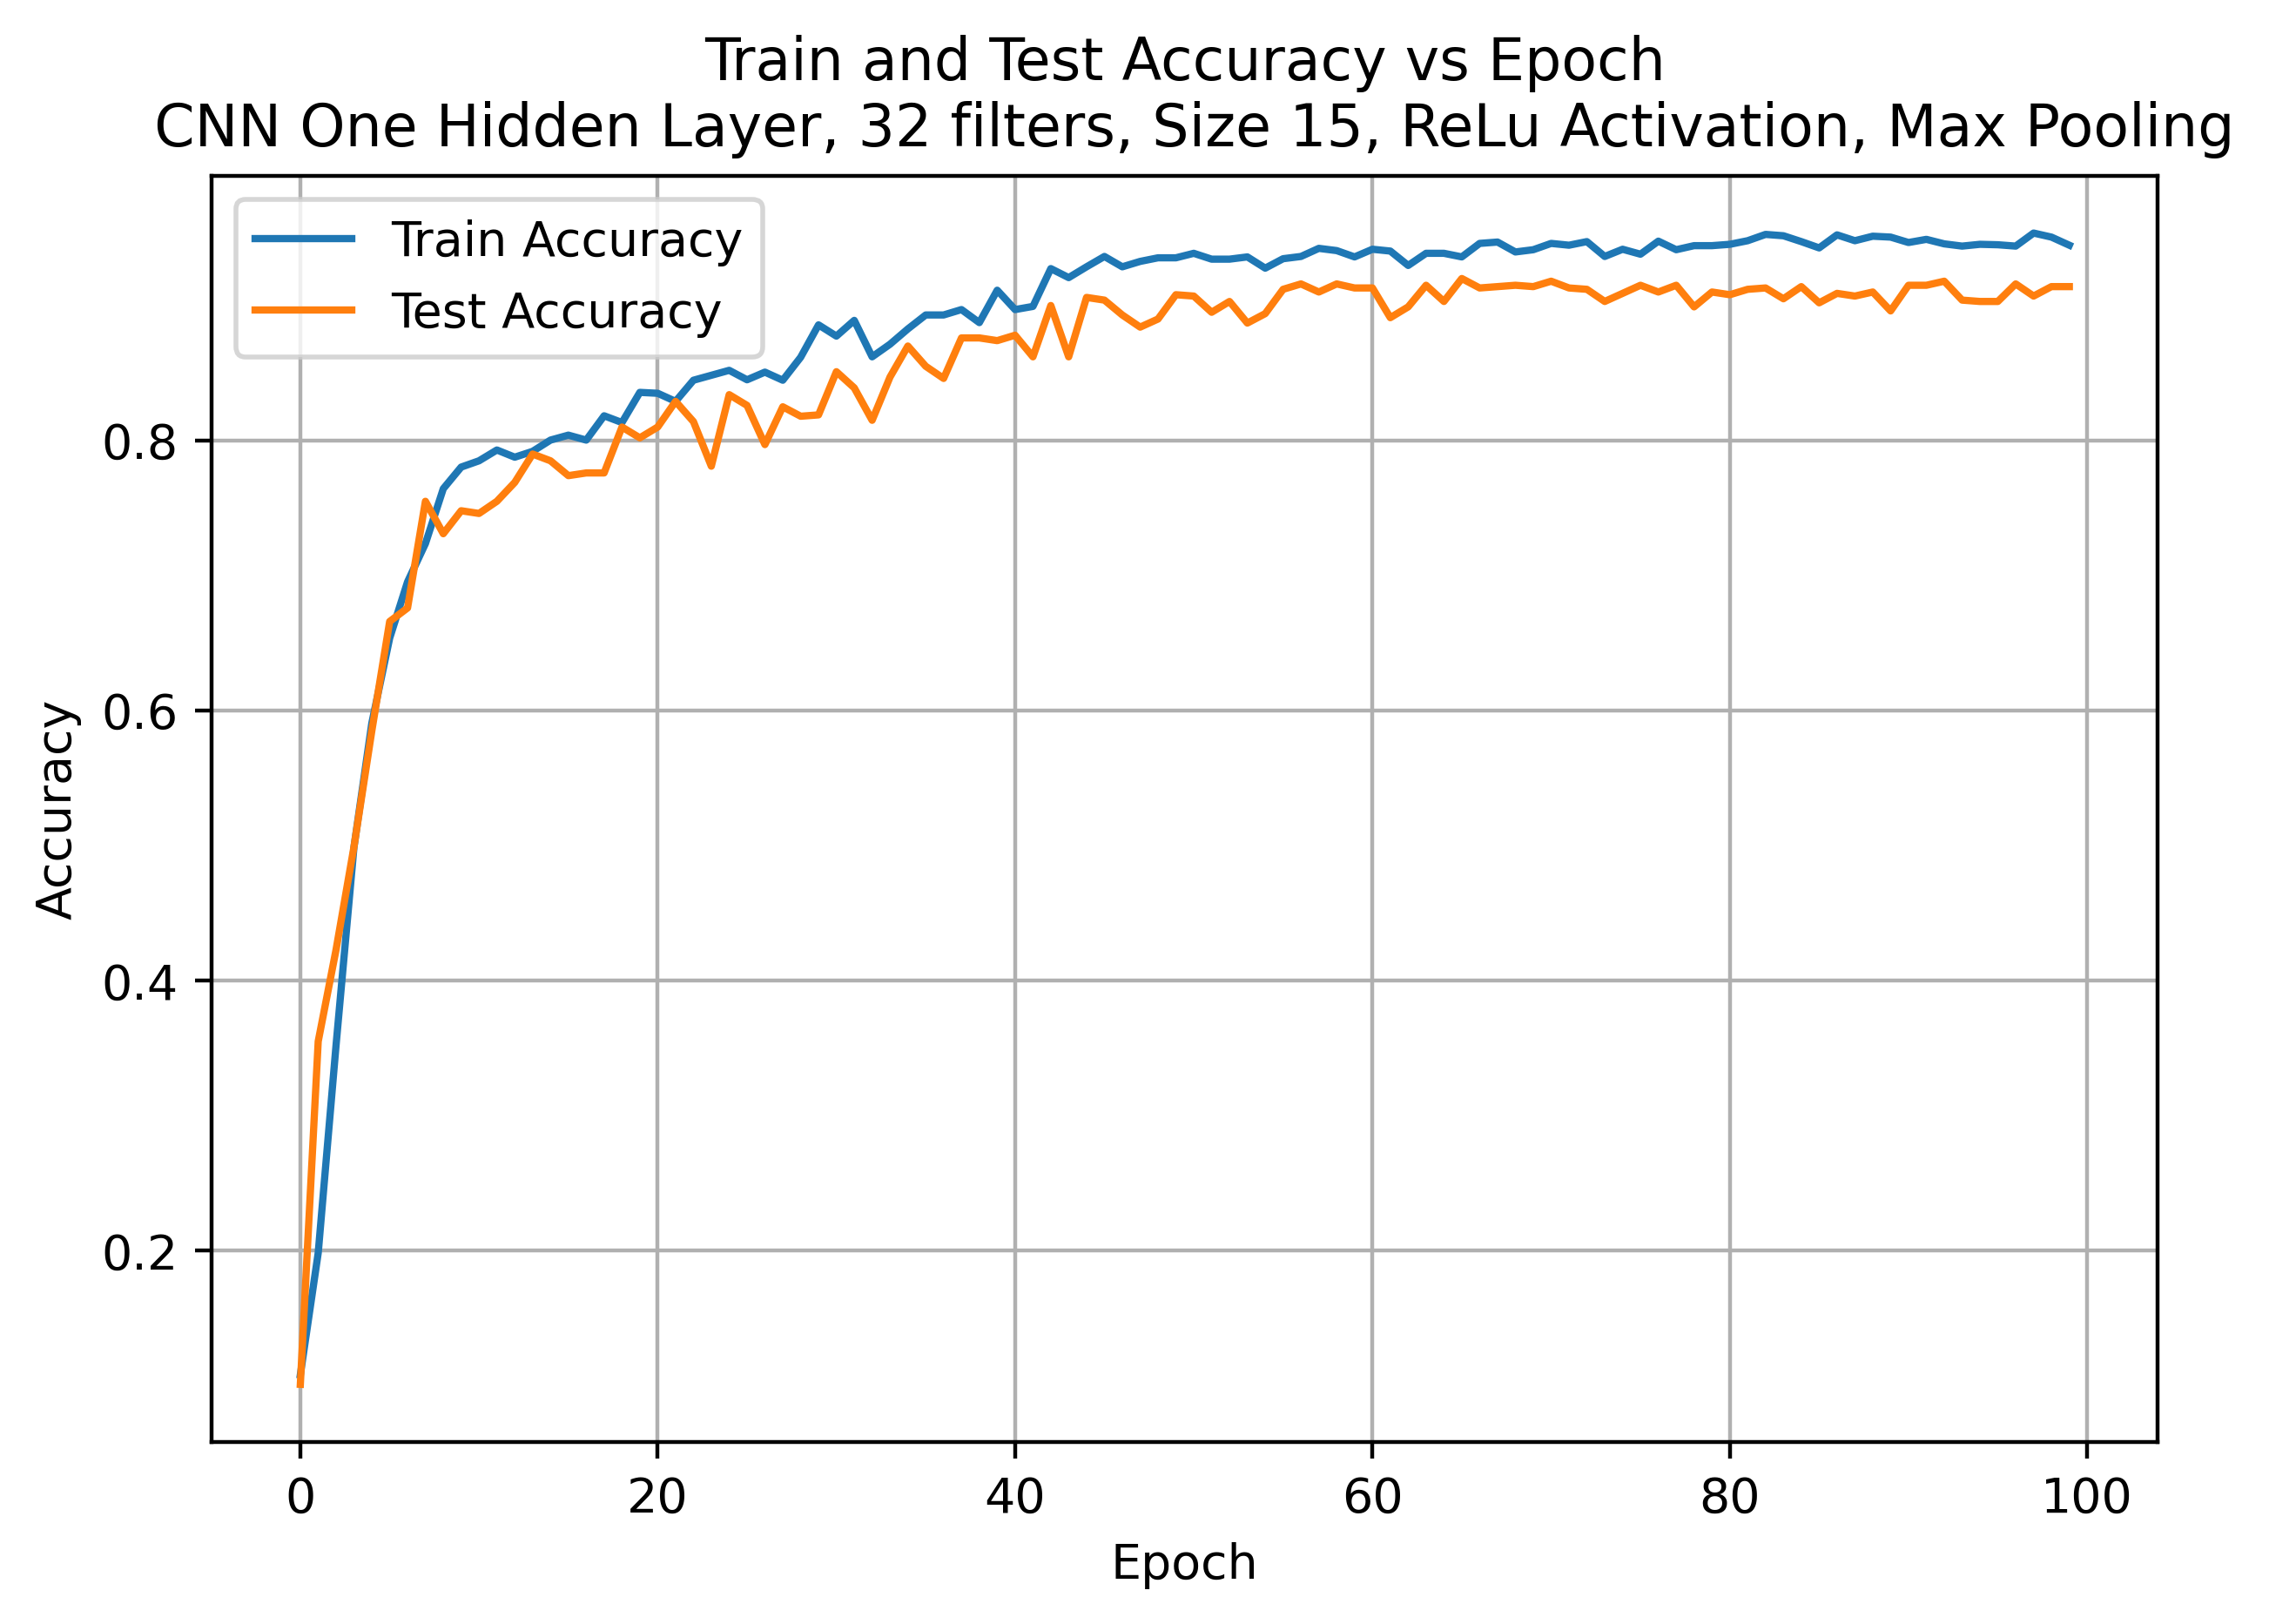
\includegraphics[width=0.5\linewidth]{../figures/part_e.png} 
        \caption{Train and Test accuracy vs. Epoch, part e.} 
    \label{fig:part e} 
    \end{figure}
    \item CNN w/ two hidden layers, 16 filters of size 15, ReLUE activation, max pooling size 2, stride 2.
    \item CNN w/ three hidden layers, 16 filters of size 15, ReLUE activation, max pooling size 2, stride 2.
\end{enumerate}

% \newpage
% \newpage
% %adding code
% \appendix
% \section*{Code}
% \lstinputlisting[language=Python]{../code/hw06.py}

\end{document}